\subsection{Excercise UseCaseDiagram CarRental}
\label{sec:exercise_use_case_diagram_car_rental}
The general functionality of the application CarRental is outlined by Alice's Car Rental story as described in \cite{CM-T-GO} listing 3.1.
It provides a general overview of the application and the user flow of registering and renting a car.

By using the story, the use cases and actors can be derived.
The following tasks are based on the story and help derive the use cases, actors and services modeled in the use case diagram.

\subsubsection*{Derive Use Cases and Actors}
The goal of this task is to find four use cases and one actor according to the given story "Alice's Car Rental" from listing 3.1 in \cite{CM-T-GO}.

% //TODO: Herleitung der vier Use Cases beschreiben
\autoref{lst:car_rental_use_case_1} was derived from line 4 of the given story.

In the story Alice rents a car, a VW ID.2, for a certain period.
This is done by entering the rental period and choosing the car from the list of available cars.

After successfully renting the car, the customer is prompted with a rental confirmation and the rental is stored.

\begin{lstlisting}[
    caption={Use Case 1: "Rent a Car"},
    label={lst:car_rental_use_case_1},
    style=kit-cm,
]
Title: Rent a Car
Primary Actor: Customer
Secondary Actor: None

Preconditions:
    - Customer is registered and logged in
    - Customer has a valid driver's license and credit card

Postconditions:
    - Customer has rented a car for the chosen time interval

Flow:
1. The customer calls the application CarRental.
2. The customer enters a start date and end date as the rental period
3. The system shows a list of the cars that are available at the selected rental period
4. The customer selects one of the listed cars
5. The system shows a rental confirmation and stores the rental

Alternative flows:
3a. no cars are available at the selected time interval
    3a1. The system shows a message that no cars are available at the selected time interval and the flow continues from 2 or terminates
4a. The customer does not want to rent any of the offered cars
    4a1. The flow terminates    
\end{lstlisting}

\autoref{lst:car_rental_use_case_2} describes the registration process itself.

It was derived from line 3 of the given story.
In order to use the application, Alice needs to register first.

After successfully registering, Alice can log in to the application and rent a car.

\begin{lstlisting}[
    caption={Use Case 2: "Registering Process"},
    label={lst:car_rental_use_case_2},
    style=kit-cm,
]
Title: Registering Process
Primary Actor: Customer
Secondary Actor: None

Preconditions:
    - The customer is not registered yet
    - Customer has a valid email address
    - Customer has a valid credit card and driver's license
    - Customer is at least 18 years old
    - Customer is not blacklisted by the car rental company or an insurance company

Postconditions:
    - Customer is registered
    - Customer can rent a car
    - Customer can log in to the car rental company's website

Flow:
1. Customer visits the car rental company's website or opens the app 
2. Customer is asked to register or login
3. Customer clicks on "Register"
4. Customer is prompted for email, name, driver's license, credit card number, date of birth
5. A data validation is performed
6. Customer needs to authenticate his email address
7. Customer chooses a password and a username
8. Customer shows a registration confirmation and the customer is registered successfully 

Alternative flows:
3a. Customer is already registered and clicks on "Login" instead of "Register"
5a. Customer prompts false information or leaves nonoptional fields empty, so the data validation fails
    5a1. The customer is asked to fill out the form again
6a. Customer does not authenticate his email address
    6a1. The customer will not be registered and the registration process will be aborted
7a. Customer chooses a username that is already taken
    7a1. The customer is asked to choose another username
7b. The provided password does not fulfill the given criteria
    7b1. The customer is asked to choose a stronger password
\end{lstlisting}

There are two types of cancellation: Cancellation of a rental and cancellation of the registration.
\autoref{lst:car_rental_use_case_3} describes the cancellation of a rental as described in lines 5 and 6 of the given story.

Like Alice in the story, the customer can cancel a rental if he successfully rented a car but does not want to use it anymore.
The customer can cancel the rental as long as the time interval of the rental has not started yet.

After successfully canceling the rental, the customer is prompted with a cancellation confirmation.

\begin{lstlisting}[
    style=kit-cm,
    caption={Use Case 3: "Cancellation of a Rental"},
    label={lst:car_rental_use_case_3},
]
Title: Cancellation of a Rental
Primary Actor: Customer
Secondary Actor: None

Preconditions:
    - Customer has rented a car
    - Customer is logged in
    - The time interval of the rental has not started yet

Postconditions:
    - Customer has cancelled the rental
    - Customer is prompted with a cancellation fee if necessary

Flow:
1. Customer calls the application CarRental
2. Customer clicks on "My Rentals"
3. Customer selects the rental he wants to cancel
4. Customer clicks on "Cancel Rental"
5. Customer is prompted with a cancellation fee if necessary
6. Customer confirms the cancellation
7. Customer is asked to confirm the cancellation again via email
8. Customer confirms the cancellation via email
9. Customer is prompted with a cancellation confirmation

Alternative flows:
3a. Customer has no rentals
    3a1. The system shows a message that the customer has no rentals and the flow terminates
4a. Customer does not want to cancel the rental and the flow terminates
5a. Customer does not want to pay the cancellation fee
    5a1. The flow terminates and the rental is not canceled
8a. Customer does not confirm the cancellation via email
    8a1. The flow terminates and the rental is not canceled
\end{lstlisting}

\autoref{lst:car_rental_use_case_4} describes the cancellation of the registration as described in line 6 of the given story.

In the story, Alice cancels her registration due to personal reasons.
The customer can cancel the registration if he does not want to use the application anymore.

After successfully canceling the registration, the customer is prompted with a cancellation confirmation and can neither log in nor use the application without registering again.

\begin{lstlisting}[
    caption={Use Case 4: "Cancellation of the Registration"},
    label={lst:car_rental_use_case_4},
    style=kit-cm,
]
Title: Cancellation of the Registration
Primary Actor: Customer
Secondary Actor: None

Preconditions:
    - Customer is registered
    - Customer is logged in
    - Customer has no rentals or outstanding payments

Postconditions:
    - Customer is not registered anymore

Flow:
1. Customer calls the application CarRental
2. Customer clicks on "My Account"
3. Customer clicks on "Cancel Registration"
4. Customer confirmes the cancellation
5. Customer is asked to confirm the cancellation again via email
6. Customer confirms the cancellation via email
7. Customer is prompted with a cancellation confirmation

Alternative flows:
3a. Customer has outstanding payments or rentals
    3a1. The system shows a message that the customer has outstanding payments or rentals and the flow terminates
4a. Customer does not want to cancel the registration and the flow terminates
6a. Customer does not confirm the cancellation via email
    6a1. The flow terminates and the registration is not canceled
\end{lstlisting}

\subsection*{Modelling the Use Case Diagram with UMLet}
The installation of the standalone version of UMLet is carried out as follows:
\begin{enumerate}
    \item Download the latest version of UMLet from \url{https://www.umlet.com/changes.htm}
    \item Extract the downloaded archive
    \item Run the executable file \texttt{umlet.sh} in the extracted folder
\end{enumerate}

A screen dump of the folder structure of the extracted archive is shown in \autoref{fig:umlet_folder_structure}.
\begin{figure}
    \centering
    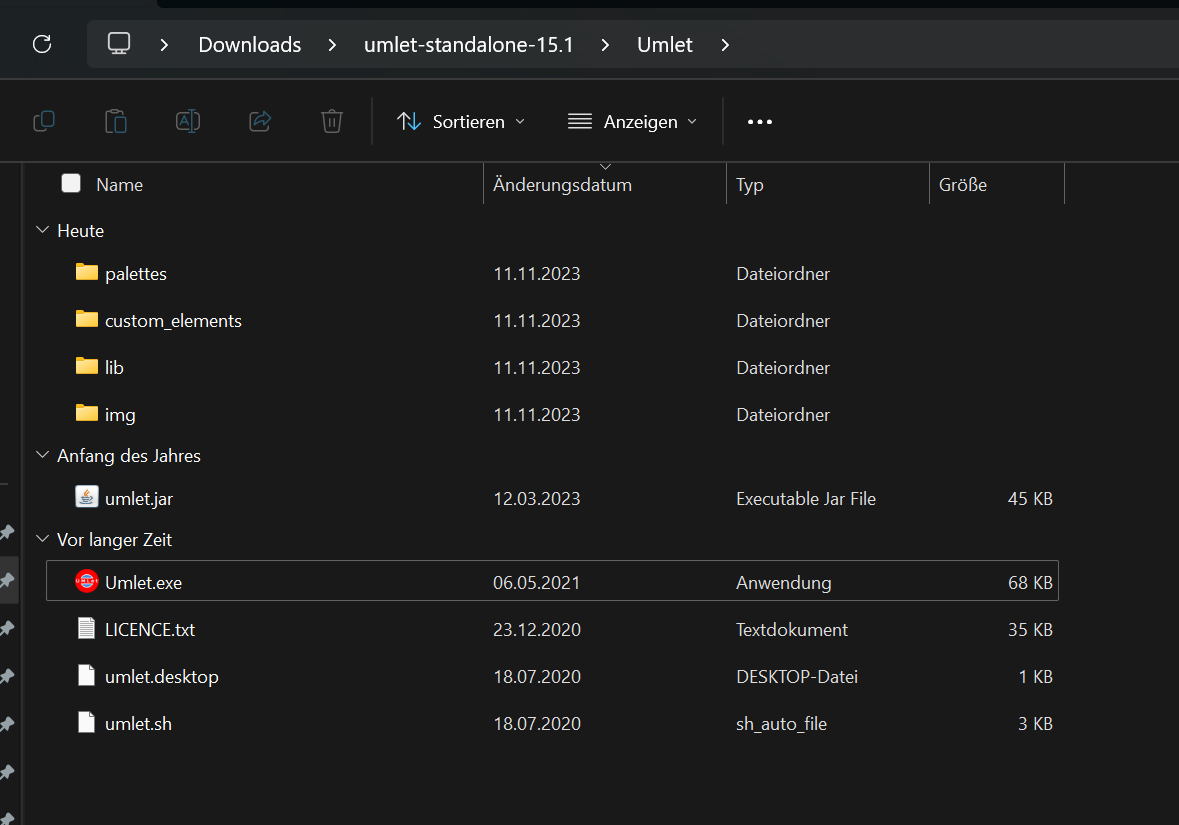
\includegraphics[width=0.8\textwidth]{figures/goLang/carRental/carRental_umletInstallation.png}
    \caption{Folder structure of the extracted UMLet archive}
    \label{fig:umlet_folder_structure}
\end{figure}

The use case diagram is shown in \autoref{fig:car_rental_use_case_diagram}.

It uses so-called services to abstract the implementation of the application.
By providing services, the implementation of the application can be changed without changing the use cases.

The registration service is used to register a customer.
It provides the user interface and structures to interact with the customer.
The registration service itself uses the authentification service to provide the customer with a secure way to authenticate himself, for example by two-factor authentification.
It also uses the cancellation service to cancel the registration if the customer wants to do so.

The rental service is used to rent a car.
It interacts with the location service, providing the location of the customer and the cars and displaying it on a map.
It also uses the cancellation service to cancel the rental if the customer wants to do so.
The car usage service is used to provide the customer with information about the car, for example, if the car is available, the current fuel level or the current mileage.

The services' interactions are displayed in the use case diagram utilizing the arrows and the corresponding labels.
\begin{figure}[H]
    \centering
    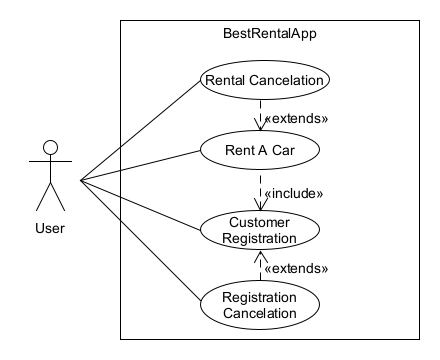
\includegraphics[width=0.8\textwidth]{figures/goLang/carRental/carRental_umlDiagram.png}
    \caption{Use case diagram of the car rental application}
    \label{fig:car_rental_use_case_diagram}
\end{figure}

\subsection{Excercise UseCase RentACar}
\label{sec:exercise_use_case_rent_a_car}
\subsubsection*{Alice's Car Rental}
This task aims to complete the use-case story "Rent a Car" for Alice.
This is done by adding the given data from the story to the use-case story.

The completed use-case story is shown in \autoref{lst:alices_car_rental_use_case_1}.

\begin{lstlisting}[
style=kit-cm,
caption={Alice's Version of Use Case 1},
label={lst:alices_car_rental_use_case_1},
]
1. Alice calls the application CarRental.
2. Alice enters 01.01.00 as a start date and 02.02.00 as the end date as the rental period
3. The system shows a list of the cars that are available at the selected rental period
4. Alice selects a VW ID.2
5. The system shows a rental confirmation and stores the rental

Alternative flows:
3a. The VW ID.2 is not available at the selected time interval
    3a1. The system shows a message that the VW ID.2 is not available at the selected time interval and the flow continues from step 2 or terminates
4a. Alice does not want to rent the VW ID.2
    4a1. The flow terminates
\end{lstlisting}
